\documentclass{article}

% if you need to pass options to natbib, use, e.g.:
% \PassOptionsToPackage{numbers, compress}{natbib}
% before loading nips_2016
%
% to avoid loading the natbib package, add option nonatbib:
% \usepackage[nonatbib]{nips_2016}

% \usepackage{nips_2016}

% to compile a camera-ready version, add the [final] option, e.g.:
\usepackage[final]{nips_2016}

\usepackage[utf8]{inputenc} % allow utf-8 input
\usepackage[T1]{fontenc}    % use 8-bit T1 fonts
\usepackage{hyperref}       % hyperlinks
\usepackage{url}            % simple URL typesetting
\usepackage{booktabs}       % professional-quality tables
\usepackage{amsfonts}       % blackboard math symbols
\usepackage{nicefrac}       % compact symbols for 1/2, etc.
\usepackage{microtype}      % microtypography

\usepackage{enumitem}
\usepackage{xfrac}

\usepackage{amsmath}
\usepackage{color}
\newcommand{\JY}[1]{\textcolor{blue}{#1}}
\usepackage{float}
\usepackage{subcaption}
\usepackage{bm}

\title{Object Detection and Orientation Estimation for Autonomous Driving}

% The \author macro works with any number of authors. There are two
% commands used to separate the names and addresses of multiple
% authors: \And and \AND.
%
% Using \And between authors leaves it to LaTeX to determine where to
% break the lines. Using \AND forces a line break at that point. So,
% if LaTeX puts 3 of 4 authors names on the first line, and the last
% on the second line, try using \AND instead of \And before the third
% author name.

\author{
  Jinyi Lu \\
  Information Networking Institute \\
  \texttt{jinyil@andrew.cmu.edu} \\
  \And
  Xiaoqing Tao \\
  Information Networking Institute\\
  \texttt{xtao@andrew.cmu.edu} \\
}

\begin{document}
\bibliographystyle{unsrt}
\maketitle

% \begin{abstract}
% No abstract.
% \end{abstract}

\textbf{Keywords:} [computer vision, object detection, object orientation estimation, autonomous driving]

% \section*{Instructions}

Your midway report should be 4 pages long (excluding references) and include the following:

\begin{itemize}[leftmargin=2em]
    \item Project title and list of group members (please follow the given template).

    \item \textbf{Introduction (1 -- 1\sfrac{1}{2} pages):}
    Problem and literature overview; how your idea fits into the existing work.
    If you already had an elaborate proposal, you may borrow this part from there, but try to make it as focused and concise as possible.
    If your proposal did not include enough background information, please make sure this section fills that gap (this will also save you time on preparing the final report).

    \item \textbf{Methods (1\sfrac{1}{2} -- 2 pages):}
    If you are developing a new method / model / architecture, this section should contain all the math, derivations, formal details, illustrations (if necessary).
    If you are proving theorems, assumptions and theorem formulations should be here.
    If your project is application driven, this section should highlight important aspects of the application and details on how your methodology addresses those.

    \item \textbf{Preliminary Results (\sfrac{1}{2} -- 1 page):}
    Please include experimental results you have obtained by the deadline.
    We expect you to have at least implemented and tested a major part of your models (maybe on some toy data) and run a few baselines.
    Describe how the current results align with your expectations.
    You may include the details on how you mined / prepared the data, if it is an important aspect of the project.

    \item \textbf{Final plan (\sfrac{1}{2} page):}
    The adjusted plan for the next steps (in terms of methodology, experiments, data collection, etc.)
\end{itemize}

\section*{Additional notes}

If you have changed or adjusted your project plan significantly (compared to what you have proposed), please provide a brief note on this in a subsection of the introduction.

\section*{Grading rubric}

\textbf{Total weight:} 25\% of the project grade (i.e., 10\% of the course grade).

\begin{itemize}[leftmargin=2em]
    \item Introduction \& literature survey (10\%)
    \item Methods (40\%)
    \item Preliminary results (20\%)
    \item Plan of the next steps (20\%)
    \item Quality of writing (10\%)
\end{itemize}

\section{Introduction}
\section{Overview}

    % \begin{itemize}
    %     \item Why the problem is important.
    %     \item What challenges you need to solve.
    %     \item Which datasets you are planning to use.
    %     \item What metrics you are planning to use to measure your performance.
    % \end{itemize}

Nowadays cameras are available onboard of of almost every new car produced in the last few years. Computer vision provides a very cost effective solution not only to improve safety, but also to one of the holy grails of AI, fully autonomous self-driving cars. 
In this project we are planning to use deep neural networks to solve the object detection and object orientation estimation problems for autonomous driving. 

There are lots of potential challenges that we need to solve for example, 
due to the road conditons, weather and car location, 
images from the car cameras will have a high-variety, which 
requires high robustness for our model. 
And besides the classical object detection task, we 
want to further estimate the 3D orientation from the 2D images.
Last, but not least our 
system need to produce a good result within a limited runtime in order 
to be used in practise.


The dataset that we are planning to use is the KITTI Vision Benchmark Suite \cite{Geiger2012CVPR}.  
It's developed for use in mobile robotics and autonomous driving research. So it 
contains several novel challenging benchmarks for the tasks of stereo, optical flow, visual
odometry/SLAM and 3D object detection. 
In our project, we mainly focus on the object detection and orientation estimation task. 
The corresponding benchmark \footnote{\url{http://www.cvlibs.net/datasets/kitti/eval_object.php}} consists of 7481 training images and 7518 test images, comprising a total of 80,256 labeled objects (up to 15 cars and 30 pedestrians are visible per image). All images are color and saved as png.

For evaluation, the benchmark is split into three parts: 
First, we need to evaluate the classical
2D object detection by measuring performance using the
well established average precision (AP) metric as described
in \cite{everingham2010pascal}.
Detections are iteratively assigned to ground truth
labels starting with the largest overlap, measured by bounding
box intersection over union. 
True positives are required 
to overlap by more than 50\% and multiple detections
of the same object are counted as false positives. 

Second, we assess the performance
of jointly detecting objects and estimating their 3D
orientation using a novel measure which is called the average
orientation similarity (AOS) \cite{Geiger2012CVPR} and is defined as:
\begin{align}
AOC & = \frac{1}{11} \sum_{r \in \{0,0.1,..,1\}} \max_{\tilde{r}:\tilde{r} \geq r} s(\tilde{r})
\end{align}

Here, $r = \frac{TP}{TP+FN}$ is the PASCAL object detection recall,
where detected 2D bounding boxes are correct if they overlap
by at least 50\% with a ground truth bounding box. The
orientation similarity $s \in [0, 1]$ at recall r is a normalized
($[0..1]$) variant of the cosine similarity defined as
\begin{align}
s(r) & = \frac{1}{|D(r)|} \sum_{i \in D(r)} \frac{1 + cos \Delta_{theta}^{(i)}}{2} \delta_i
\end{align}
where $D(r)$ denotes the set of all object detections at recall
rate 
$r$ and $\Delta_{theta}^{(i)}}$
is the difference in angle between estimated
and ground truth orientation of detection $i$. To penalize multiple
detections which explain a single object, we set $\delta_i = 1$
if detection $i$ has been assigned to a ground truth bounding
box (overlaps by at least 50\%) and $\delta_i = 0$ if it has not been
assigned.

Finally, we will also evaluate pure classification (16 bins for
cars) and regression (continuous orientation) performance
on the task of 3D object orientation estimation in terms of
orientation similarity.





\subsection{Related work}
\label{others}
Traditional methods for object detection usually utilize image features,such as SIFT and HOG. We investigated three methods utilizing deep convolutional network in object detection.
\subsection{R-CNN: Rich feature hierarchies for accurate object detection and semantic segmentation}

 The first challenge for object detection is how to implement localizing within an image. The new method proposed in this paper\cite {rcnn} combines CNN with region proposals. So it is called R-CNN. The general detection process is to extract about 2000 region proposals for each input image. Then utilize CNN to compute a fixed length feature for each region proposal. Finally utilize linear SVM to classify each region. 


The second challenge is how to train a large CNN using limited labeled data. This paper proposed to pre-train CNN on a large auxiliary data set, then continually train on a small data set. This method significantly improved the accuracy of objection detection compared with feature learning models. But training is expensive in space and time, and detection is also slow at test time.

\subsection{Fast R-CNN}
This paper\cite {fast-rcnn} talked about how to train a detection network faster. R-CNN is very slow because it extracts feature for each region proposal and there are many duplicate computations. The process could be faster if we share computation. 

This paper proposed to modify R-CNN’s architecture by taking an image and multiple regions of interests as input. Region proposal method usually depends on Selective Search. Each region of interest is pooled into a fixed-size feature map and fully connected layers are used to extract features. There two output vectors: softmax probabilities and per-class bounding-box regression offsets.The second one is to reduce mislocalization.

\subsection{Faster R-CNN: Towards Real-Time Object Detection with Region Proposal Networks}
Fast-CNN achieves near real-time rates using very deep networks, when ignoring the time spent on region proposals. Select Search takes about 2 seconds per image on the CPU. Faster R-CNN\cite {faster-rcnn} adds a fully convolutional network to compute region proposals directly. Then use the same detector on the proposed regions as what Fast R-CNN does. 

\JY{
\subsection{Yolo}
}




\section{Methods}
\section{Results}

In this section, we will discuss some of our results.
In terms of evaluating the object detection results, KITTI benchmark requires a minimum overlap of 70\% for cars and 50\% for pedestrians. It also has three kinds of difficulties: easy, moderate and hard. Difficulties are defined as follows:

\begin{table}[h!]
\centering
\begin{tabular}{ c | c | c | c }
\hline
Difficulty & Min. bounding box height & Max. occlusion level & Max. truncation \\
\hline \hline
Easy & 40 Px & Fully visible & 15\% \\
Moderate & 25 Px & Partly occluded & 30\% \\
Hard & 25 Px & Difficult to see & 50\% \\
\hline
\end{tabular}
\caption{Different Difficulties Requirements}
\end{table}


Originally, we used all the data we have. 
However, since training on the whole set takes lots of time, 
we only work on a subset of all the data (about 30\%).

\subsection{Subset Sampling}
We have 7841 labeled images in total with about 80,256 labeled 
objects. However, in order to speed up the development process, 
we choose to only use 30\% of all the images we have (1637 images for training and 828 images for validation) and detect two 
kinds of object: car and pedestrians.

\begin{table}[h!]
\centering
\begin{tabular}{ c | c | c }
\hline
Object & Avg Number of Object (Whole Set) & Avg Number of Object (Subset)\\ 
\hline \hline
Car & 3.8429 & 3.8502\\
Pedestrians & 0.5998 & 0.6630\\
\hline
\end{tabular}
\caption{Average Number of Objects Per Image}
\end{table}

Previously, we have conducted two experiments on the whole dataset,
including using a pre-trained yolo model,
and using a pre-trained Faster-RCNN model. All the experiments are conducted on AWS using a p2.xlarge instance with Tesla K80 GPU. We directly use the Yolo implementation from Darknet \footnote{\url{https://github.com/pjreddie/darknet.git}} and the Faster R-CNN python implementation \footnote{\url{https://github.com/rbgirshick/py-faster-rcnn}}.

The pre-trained yolo model is trained on Pascal VOC 2012 and 2007 dataset \footnote{\url{http://pjreddie.com/darknet/yolo/}}. It supports about 20 object categories including car and people (corresponding to pedestrian). However it don't support cyclist category. So in all the following experiments, we only evaluate the performance for cars and pedestrians.

The pre-trained Faster-RCNN model is trained on Pascal VOC 2007 dataset. It is able to detect cars and pedestrians and also lacks of supports for cyclists.

So next we will compare their performance on the subset with the 
previous results to see whether the subset sampling affects the 
model performance.


\begin{figure}[h!]
\centering
\begin{subfigure}[t]{.24\textwidth}
    \centering
    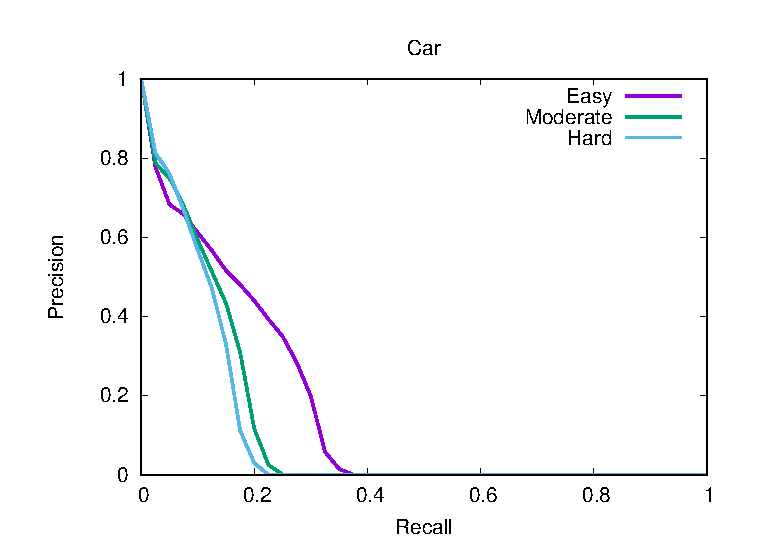
\includegraphics[width=1.0\linewidth]{img/yolo_Nov_4/plot_valid/car_detection.eps}
    \caption{Pre-Trained Yolo on Whole Set}
\end{subfigure}
\begin{subfigure}[t]{.24\textwidth}
    \centering
    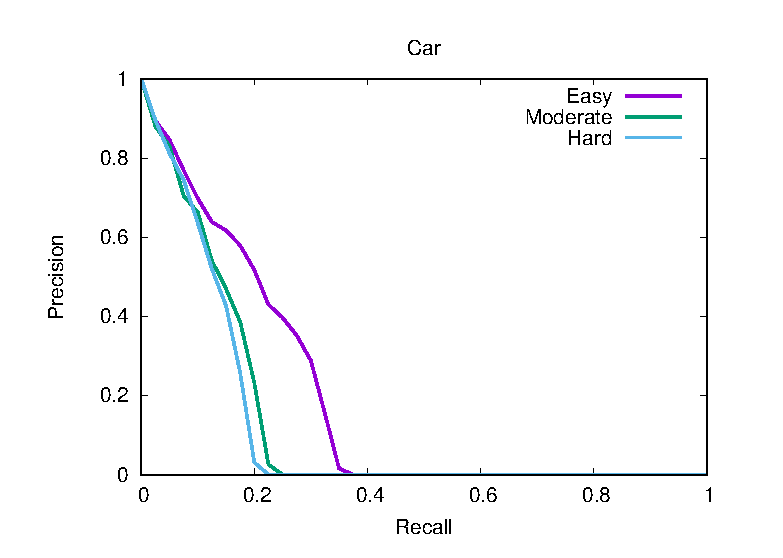
\includegraphics[width=1.0\linewidth]{img/yolo_Nov_4/plot_valid_30/car_detection.eps}
    \caption{Pre-Trained Yolo on Subset}
\end{subfigure}
\begin{subfigure}[t]{.24\textwidth}
    \centering
    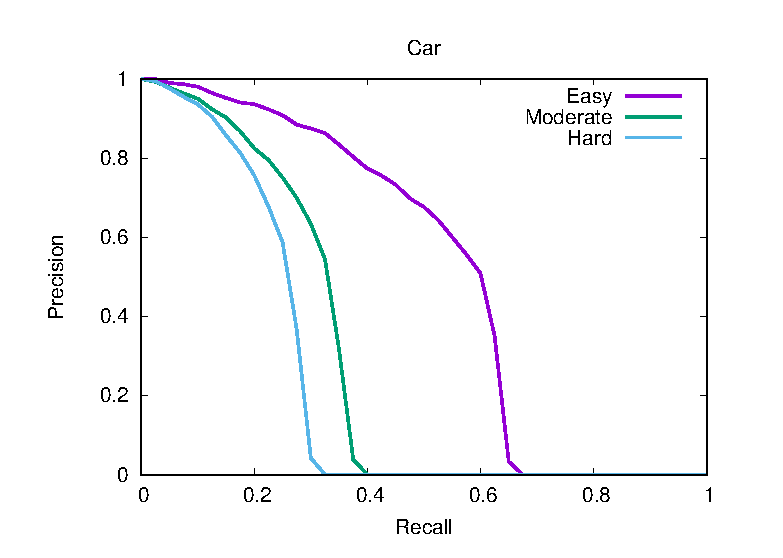
\includegraphics[width=1.0\linewidth]{img/FRCNN_Nov_8/plot_valid/car_detection.eps}
    \caption{Pre-Trained Faster-RCNN on Whole Set}
\end{subfigure}
\begin{subfigure}[t]{.24\textwidth}
    \centering
    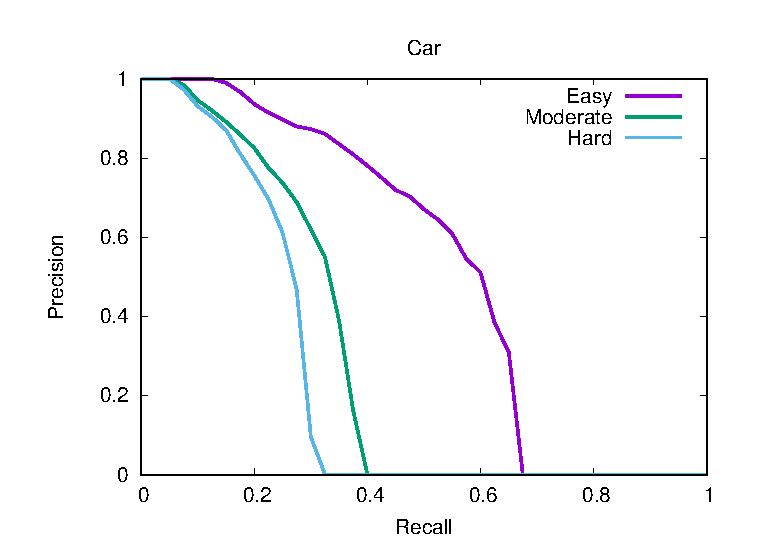
\includegraphics[width=1.0\linewidth]{img/FRCNN_Nov_8/plot_valid_30/car_detection.eps}
    \caption{Pre-Trained Faster-RCNN on Subset}
\end{subfigure}
\caption{Car Detection}
\end{figure}

\begin{table}[h!]
\centering
\begin{tabular}{ c | c | c | c }
\hline
Method & Easy & Moderate & Hard \\
\hline \hline
Pre-Trained Yolo Whole Set & 0.204438 & 0.155358 & 0.145101 \\
Pre-Trained Yolo Subet & 0.227639 & 0.172312 & 0.151478 \\
Pre-Trained Faster-RCNN Whole Set & 0.522754 & 0.309875 & 0.248554 \\
Pre-Trained Faster-RCNN Subet & 0.524807 & 0.308296 & 0.252989 \\
\hline
\end{tabular}
\caption{Average Precision on Car Detection}
\end{table}


\begin{figure}[H]
\centering
\begin{subfigure}[t]{.24\textwidth}
    \centering
    \includegraphics[width=1.0\linewidth]{img/yolo_Nov_4/plot_valid/pedestrian_detection.eps}
    \caption{Pre-Trained Yolo on Whole Set}
\end{subfigure}
\begin{subfigure}[t]{.24\textwidth}
    \centering
    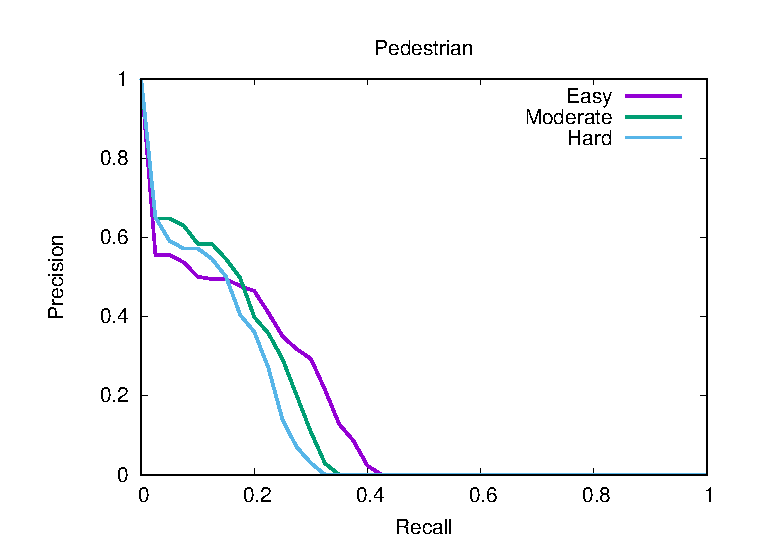
\includegraphics[width=1.0\linewidth]{img/yolo_Nov_4/plot_valid_30/pedestrian_detection.eps}
    \caption{Pre-Trained Yolo on Subset}
\end{subfigure}
\begin{subfigure}[t]{.24\textwidth}
    \centering
    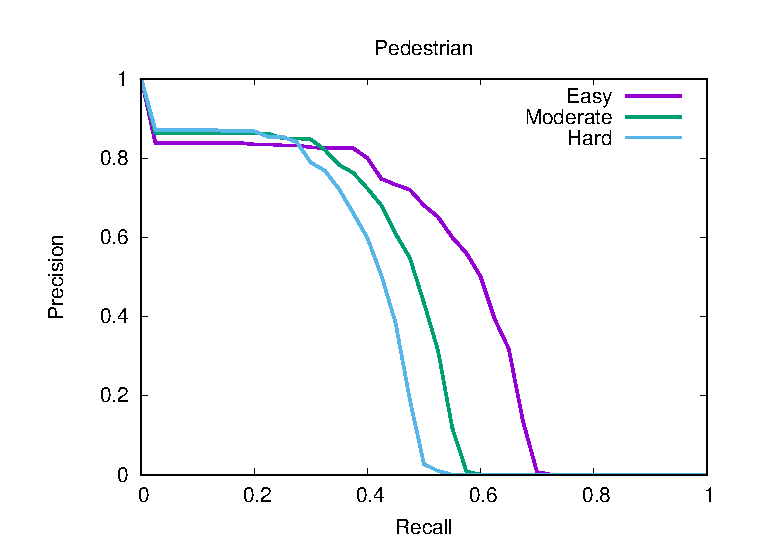
\includegraphics[width=1.0\linewidth]{img/FRCNN_Nov_8/plot_valid/pedestrian_detection.eps}
    \caption{Pre-Trained Faster-RCNN on Whole Set}
\end{subfigure}
\begin{subfigure}[t]{.24\textwidth}
    \centering
    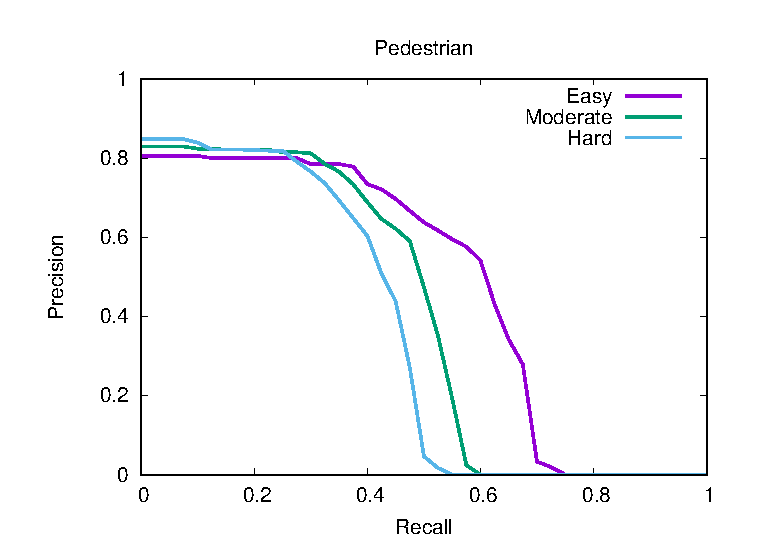
\includegraphics[width=1.0\linewidth]{img/FRCNN_Nov_8/plot_valid_30/pedestrian_detection.eps}
    \caption{Pre-Trained Faster-RCNN on Subset}
\end{subfigure}
\caption{Pedestrian Detection}
\end{figure}

\begin{table}[h!]
\centering
\begin{tabular}{ c | c | c | c }
\hline
Method & Easy & Moderate & Hard \\
\hline \hline
Pre-Trained Yolo Whole Set & 0.197457 & 0.183323 & 0.175022 \\
Pre-Trained Yolo Subet & 0.207263 & 0.189966 & 0.178328 \\
Pre-Trained Faster-RCNN Whole Set & 0.498992 & 0.429862 & 0.377569 \\
Pre-Trained Faster-RCNN Subet & 0.467467 & 0.404372 & 0.356576 \\
\hline
\end{tabular}
\caption{Average Precision on Car Detection}
\end{table}

As we can see, the performance of those two models doesnt' have 
significant difference on the subset compare with the whole set. 
So in all the following experiments, we only work on the subset.

\subsection{Convergence Properties of Different Models}
We build four fine-tuned models, which are
tiny yolo, big yolo, Faster R-CNN using ZFnet and 
Faster-RCNN using VGG\textunderscore CNN\textunderscore M\textunderscore 1024 \cite{chatfield2014return}.

In this section we will show some results about 
their convergence properties by visualizing their loss/error 
changes with iterations.

\begin{figure}[H]
\centering
\begin{subfigure}[t]{.49\textwidth}
    \centering
    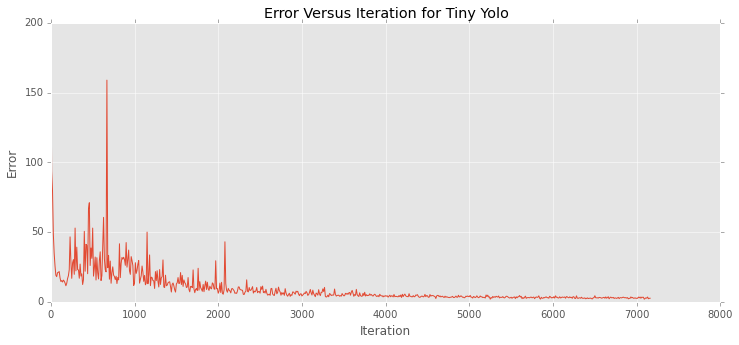
\includegraphics[width=1.0\linewidth]{img/yolo_tiny_cov.png}
    \caption{Tiny Yolo}
\end{subfigure}
\begin{subfigure}[t]{.49\textwidth}
    \centering
    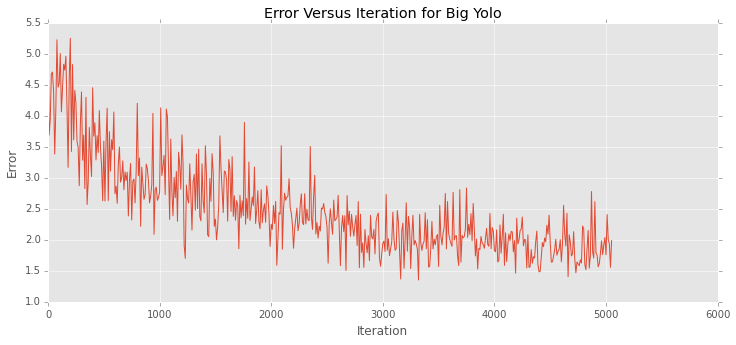
\includegraphics[width=1.0\linewidth]{img/yolo_big_cov.png}
    \caption{Big Yolo}
\end{subfigure}
\caption{Convergence Properties of Yolo}
\end{figure}

\begin{figure}[H]
\centering
\begin{subfigure}[t]{.49\textwidth}
    \centering
    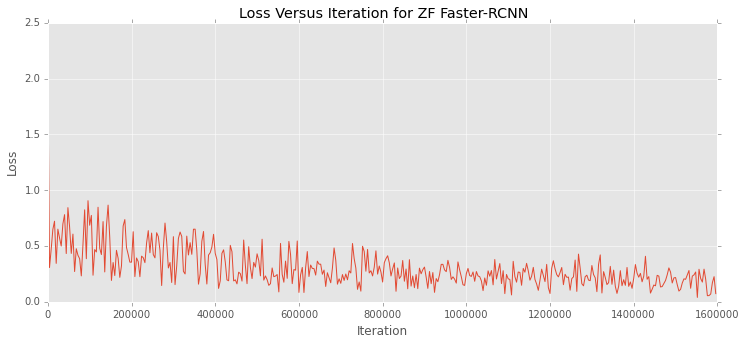
\includegraphics[width=1.0\linewidth]{img/FRCNN_zf_cov.png}
    \caption{Faster R-CNN using ZFnet for Feature Map}
\end{subfigure}
\begin{subfigure}[t]{.49\textwidth}
    \centering
    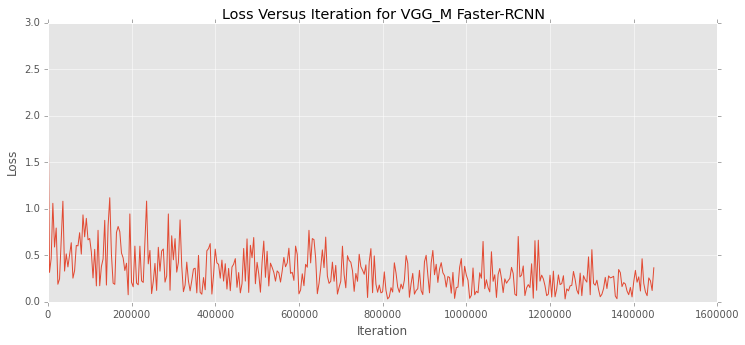
\includegraphics[width=1.0\linewidth]{img/FRCNN_vgg_m_cov.png}
    \caption{Faster R-CNN using VGG\textunderscore CNN\textunderscore M\textunderscore 1024 for Feature Map}
\end{subfigure}
\caption{Convergence Properties of Faster R-CNN}
\end{figure}

As we can see, all the models are very hard to converge even 
with their carefully designed adapting learning rates. 


\subsection{Fine-Tuned Models with Different Network Structure}
In this experiments, we test four different models which has 
different network structure.
A tiny yolo model is a simplified version of the big yolo model 
by reducing 16 convolutional layers for generating features. 
And the difference between two Faster R-CNN models
is using which convolutional networks for generating feature map,
one is ZFnet \cite{zeiler2014visualizing} and the other one is VGG\textunderscore CNN\textunderscore M\textunderscore 1024 \cite{chatfield2014return}. These two convolutional networks 
are quite similar except that 
VGG\textunderscore CNN\textunderscore M\textunderscore 1024 
is wider than ZFnet.

We use convolutional weights that are pre-trained on ImageNet classification task as initial weights. Fine tuning models make it possible to benefit from the features the model has learnt previously and speed up training. 

It took about 5 hours to train a tiny yolo after 5,000 iterations
and 15 hours to train a big yolo after 5,000 iterations.
For Faster R-CNN, the one using ZFnet took about 16 hours after 
80,000 iterations and the one using VGG\textunderscore CNN\textunderscore M\textunderscore 1024
took about 12 hours after 80,000 iterations.



\begin{figure}[h!]
\centering
\begin{subfigure}[t]{.32\textwidth}
    \centering
    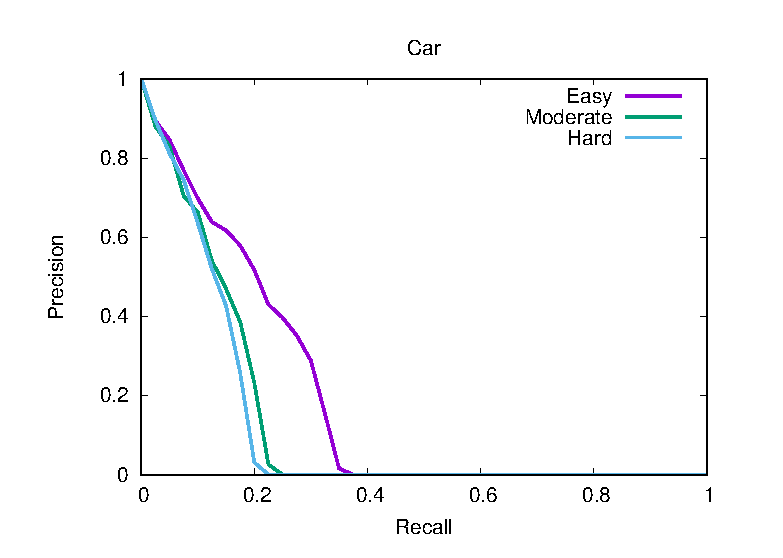
\includegraphics[width=1.0\linewidth]{img/yolo_Nov_4/plot_valid_30/car_detection.eps}
    \caption{Pre-Trained Yolo}
\end{subfigure}%
\begin{subfigure}[t]{.32\textwidth}
    \centering
    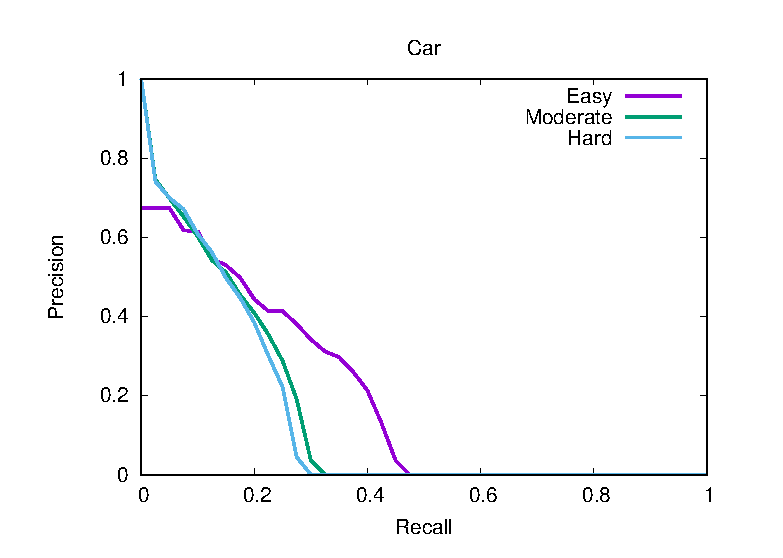
\includegraphics[width=1.0\linewidth]{img/yolo_Dec_7_tiny/plot_valid_30/car_detection.eps}
    \caption{Fine-Tuned Tiny Yolo}
\end{subfigure}%
\begin{subfigure}[t]{.32\textwidth}
    \centering
    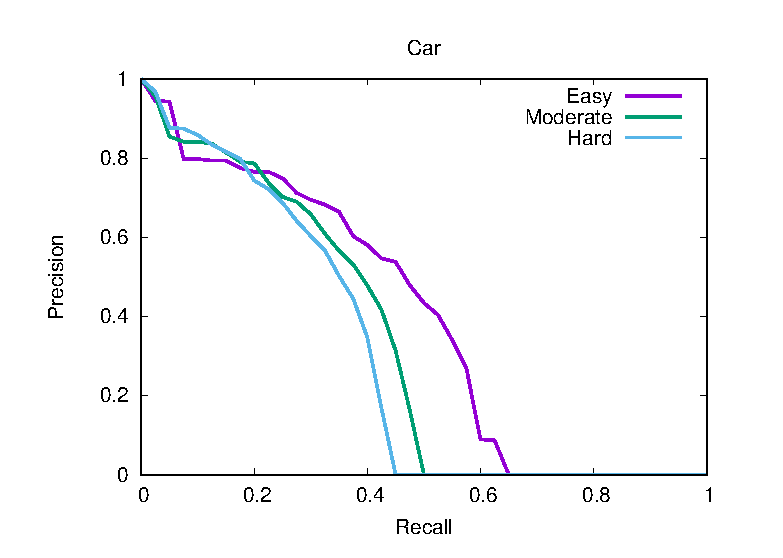
\includegraphics[width=1.0\linewidth]{img/yolo_Dec_7_big/plot_valid_30/car_detection.eps}
    \caption{Fine-Tuned Big Yolo}
\end{subfigure}
\begin{subfigure}[t]{.32\textwidth}
    \centering
    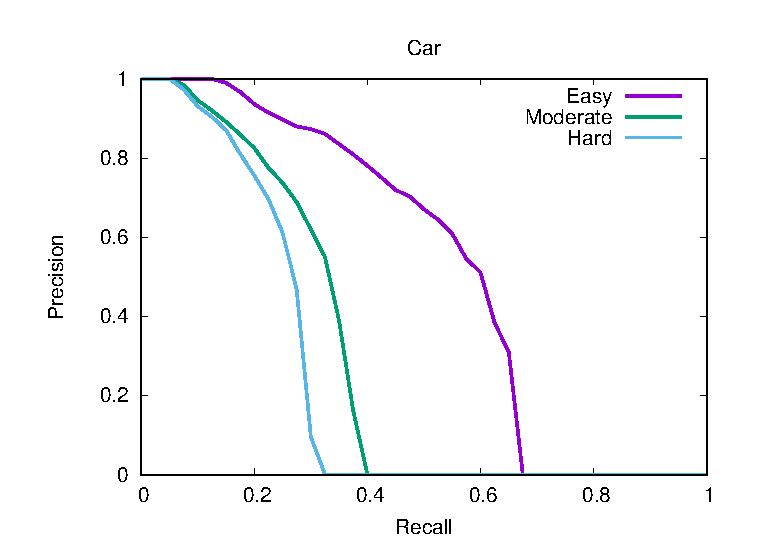
\includegraphics[width=1.0\linewidth]{img/FRCNN_Nov_8/plot_valid_30/car_detection.eps}
    \caption{Pre-Trained Faster R-CNN}
\end{subfigure}%
\begin{subfigure}[t]{.32\textwidth}
    \centering
    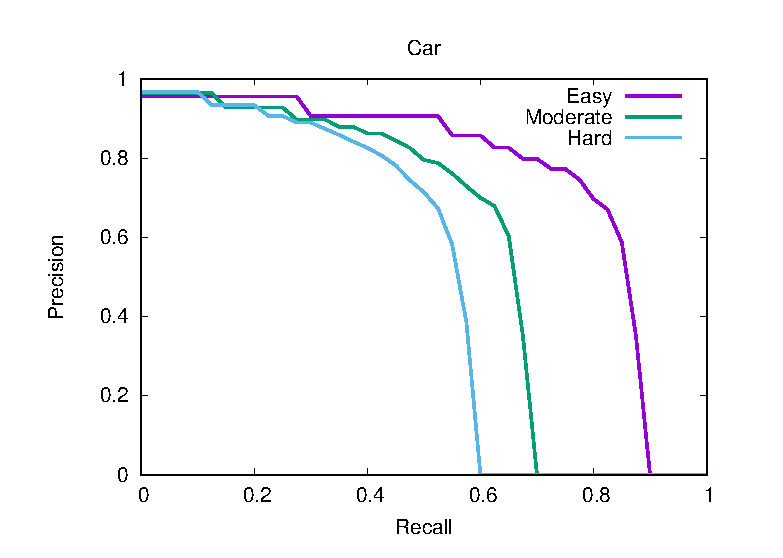
\includegraphics[width=1.0\linewidth]{img/FRCNN_Dec_7_tiny/plot_valid_30/car_detection.eps}
    \caption{Fine-Tuned Faster R-CNN using ZFnet}
\end{subfigure}%
\begin{subfigure}[t]{.32\textwidth}
    \centering
    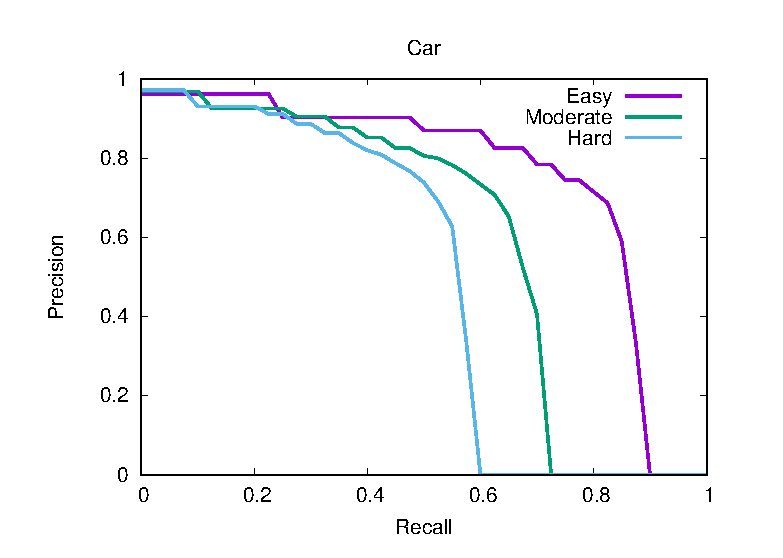
\includegraphics[width=1.0\linewidth]{img/FRCNN_Dec_7_mid/plot_valid_30/car_detection.eps}
    \caption{Fine-Tuned Faster R-CNN using VGG\textunderscore CNN\textunderscore M\textunderscore 1024 }
\end{subfigure}
\caption{Car Detection}
\end{figure}

\begin{table}[h!]
\centering
\begin{tabular}{ c | c | c | c }
\hline
Method & Easy & Moderate & Hard \\
\hline \hline
Pre-Trained Yolo & 0.227639 & 0.172312 & 0.151478 \\
Fine-Tuned Tiny Yolo & 0.207844 & 0.186021 & 0.181117 \\
Fine-Tuned Big Yolo & 0.396407 & 0.342113 & 0.322760 \\
Pre-Trained Faster R-CNN & 0.524807 & 0.308296 & 0.252989 \\
Fine-Tuned ZF Faster R-CNN & \bfseries 0.721690 & 0.555533 & \bfseries 0.481580 \\
Find-Tuned VGG\textunderscore M Faster R-CNN & 0.721039 & \bfseries 0.596753 & 0.479783 \\
\hline
\end{tabular}
\caption{Average Precision on Car Detection}
\end{table}

\begin{figure}[H]
\centering
\begin{subfigure}[t]{.32\textwidth}
    \centering
    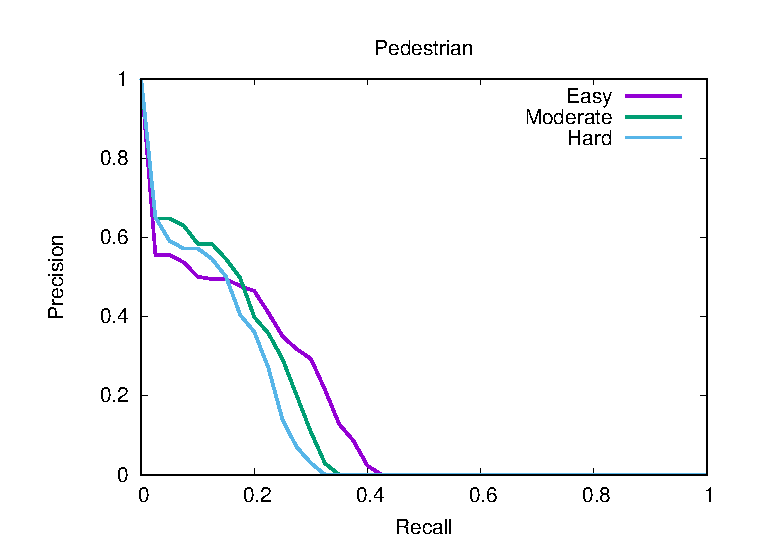
\includegraphics[width=1.0\linewidth]{img/yolo_Nov_4/plot_valid_30/pedestrian_detection.eps}
    \caption{Pre-Trained Yolo}
\end{subfigure}%
\begin{subfigure}[t]{.32\textwidth}
    \centering
    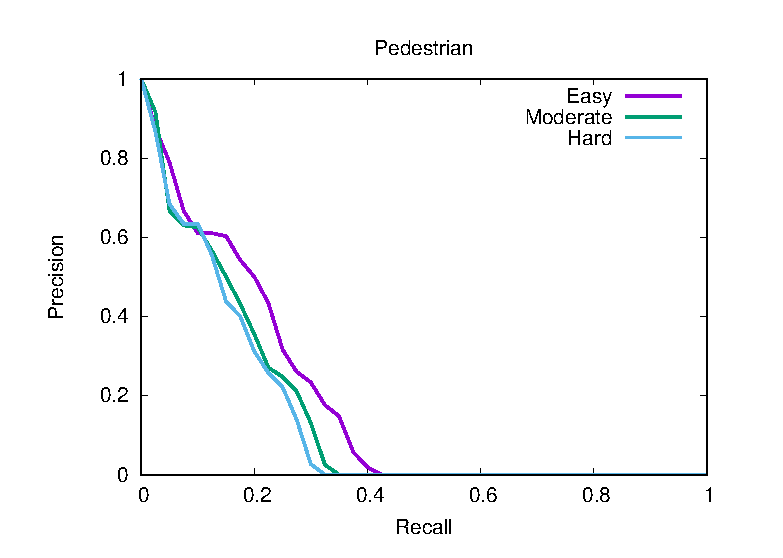
\includegraphics[width=1.0\linewidth]{img/yolo_Dec_7_tiny/plot_valid_30/pedestrian_detection.eps}
    \caption{Fine-Tuned Tiny Yolo}
\end{subfigure}%
\begin{subfigure}[t]{.32\textwidth}
    \centering
    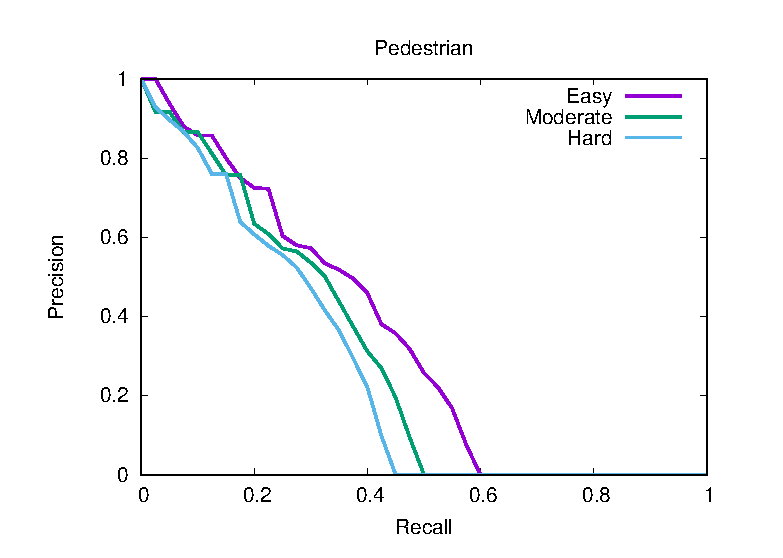
\includegraphics[width=1.0\linewidth]{img/yolo_Dec_7_big/plot_valid_30/pedestrian_detection.eps}
    \caption{Fine-Tuned Big Yolo}
\end{subfigure}
\begin{subfigure}[t]{.32\textwidth}
    \centering
    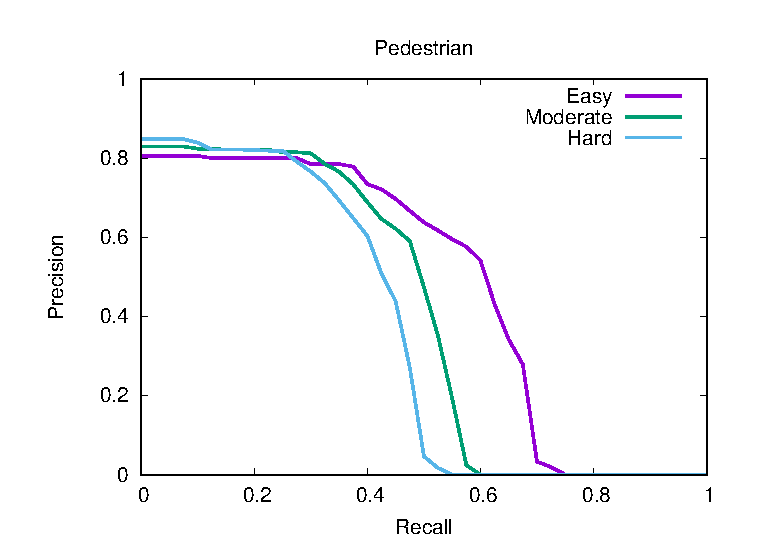
\includegraphics[width=1.0\linewidth]{img/FRCNN_Nov_8/plot_valid_30/pedestrian_detection.eps}
    \caption{Pre-Trained Faster R-CNN}
\end{subfigure}%
\begin{subfigure}[t]{.32\textwidth}
    \centering
    \includegraphics[width=1.0\linewidth]{img/FRCNN_Dec_7_tiny/plot_valid_30/pedestrian_detection.eps}
    \caption{Fine-Tuned Faster R-CNN using ZFnet}
\end{subfigure}%
\begin{subfigure}[t]{.32\textwidth}
    \centering
    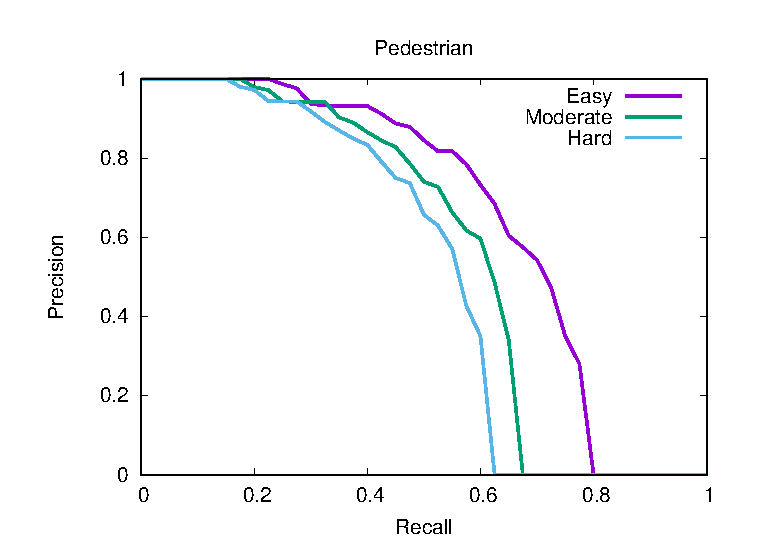
\includegraphics[width=1.0\linewidth]{img/FRCNN_Dec_7_mid/plot_valid_30/pedestrian_detection.eps}
    \caption{Fine-Tuned Faster R-CNN using VGG\textunderscore CNN\textunderscore M\textunderscore 1024 }
\end{subfigure}
\caption{Pedestrian Detection}
\end{figure}

\begin{table}[h!]
\centering
\begin{tabular}{ c | c | c | c }
\hline
Method & Easy & Moderate & Hard \\
\hline \hline
Pre-Trained Yolo & 0.207263 & 0.189966 & 0.178328 \\
Fine-Tuned Tiny Yolo & 0.214768 & 0.191912 & 0.179325 \\
Fine-Tuned Big Yolo & 0.351823 & 0.304227 & 0.284068 \\
Pre-Trained Faster R-CNN & 0.467467 & 0.404372 & 0.356576 \\
Fine-Tuned ZF Faster R-CNN &  0.621262 & 0.556017 & \bfseries 0.526138 \\
Find-Tuned VGG\textunderscore M Faster R-CNN & \bfseries 0.635249 & \bfseries 0.556700 & 0.520960 \\
\hline
\end{tabular}
\caption{Average Precision on Pedestrian Detection}
\end{table}

\subsection{Detected Object Bounding Boxes}
In this section, we explore the detected object bounding boxes by different 
models by checking the average height, width and area of detected objects. For all the models, we only consider the detected 
object with confidence heigher than 0.2.

\begin{table}[H]
\centering
\begin{tabular}{ c | c | c | c | c}
\hline
Method & Avg Height & Avg Width & Avg Area & cnt \\
\hline \hline
\bfseries Ground Truth & \bfseries 66.6599 & \bfseries 113.2698 & \bfseries 11449.9983 & \bfseries 3188 \\
Fine-Tuned Tiny Yolo & 81.4113 & 130.9231 & 14518.8764 & 2601 \\
Fine-Tuned Big Yolo & 67.6324 & 117.1498 & 11676.8592 & 3029 \\
Fine-Tuned ZF Faster R-CNN & 63.7740 & 102.8394 & 10458.8683 & 3502 \\
Find-Tuned VGG\textunderscore M Faster R-CNN & 62.7834 & 100.1970 & 9768.3991 & 3885 \\
\hline
\end{tabular}
\caption{Detected Car Bounding Boxes Comparison}
\end{table}

\begin{table}[H]
\centering
\begin{tabular}{ c | c | c | c | c}
\hline
Method & Avg Height & Avg Width & Avg Area & cnt \\
\hline \hline
\bfseries Ground Truth & \bfseries 103.2774 & \bfseries 43.3553 & \bfseries 6081.0395 & \bfseries 549 \\
Fine-Tuned Tiny Yolo & 158.6333 & 69.7682 & 12327.1655 & 235 \\
Fine-Tuned Big Yolo & 132.4591 & 64.1588 & 9822.6585 & 225 \\
Fine-Tuned ZF Faster R-CNN & 105.9067 & 45.7684 & 6179.3364 & 585 \\
Find-Tuned VGG\textunderscore M Faster R-CNN & 96.6618 & 44.1266 & 5529.7738 & 662 \\
\hline
\end{tabular}
\caption{Detected Pedestrian Bounding Boxes Comparison}
\end{table}


\subsection{Prediction Speed}
\begin{table}[H]
\centering
\begin{tabular}{ c | c}
\hline
Method & FPS \\
\hline \hline
Fine-Tuned Tiny Yolo  & 70 \\
Fine-Tuned Big Yolo & 14 \\
Fine-Tuned ZF Faster R-CNN & 4\\
Find-Tuned VGG\textunderscore M Faster R-CNN & 4\\
\hline
\end{tabular}
\caption{Prediction Speed}
\end{table}




\section{Discuss}





As we can see from the precision-recall curve and the average precision results, for pedestrians, Faster-RCNN outperforms yolo models a lot in all three difficulty levels. And a fine-tuned tiny yolo model on our dataset shows no improvement compared with the pre-trained yolo model. For cars, Faster-RCNN outperforms yolo models in easy level. And our fine-tuned tiny yolo model shows great improvement in all three difficulty levels compared with the pre-traiend yolo model. And
in terms of predicting speed, the fine-tuned tiny yolo can achieve about 70 fps and the pre-trained Faster-RCNN can only achieve about 2 fps.


It seems hard to strike a balance between speed and accuracy of detection. Yolo is extremely fast on real-time detection because it only requires a single network evaluation. But the detection accuracy is not enough. Yolo only predicts 2 bounding boxes in each grid cell and 98 bounding boxes per image. This imposes strong spatial constraints to limit the number of nearby objects that the model can predict. Yolo performs poorly in detecting small objects, especially in groups. It also struggles to localize objects correctly. The impact of a small error in a small bounding box should weigh more heavily than the impact of a small error in a large bounding. But yolo treats them as the same.

Faster RCNN is another state-of-the-art object-detecting model. It is a high-accuracy detector, outperforming yolo. It benefits from explicit region proposals. But the VGG-CNN-M-1024 version of Faster R-CNN is about 4 times slower than YOLO.

In the future, we would like to increase the speed of real-time detection on KITTI dataset without sacrificing the detection accuracy. We may try other models such as SSD. It's fundamental improvement in speed comes from eliminating bounding box proposals and the subsequent pixel or feature resampling stage. Other modifications include using a small convolutional filter to predict object categories and offsets in bounding box locations, using separate predictors (filters) for different aspect ratio detections, and applying these filters to multiple feature maps from the later stages of a network in order to perform detection at multiple scales. We hope SSD model can improve the detection on KITTI dataset.

% \section{Project Plan}
We plan to implement 2D object detection using faster R-CNN by the second milestone. After that, we will focus on 3D object detection. We may also try YOLO\cite{yolo} method and see if there are any improvement. Detailed plan depends on time and compute power.

% \subsection*{References}

% \printbibliography

\bibliography{references.bib}

\end{document}
